\chapter{Anexos}
\label{chap:anexos}

\section{Cuestionario de Evaluación y Reflexión}

A continuación, se presenta la resolución detallada del cuestionario y los temas de discusión propuestos por la cátedra al final de la guía de trabajos prácticos.

\begin{enumerate}[label=\alph*)]
    \item \textit{Si en el procedimiento para medir ganancia en dB, se ve obligado a cambiar el rango del voltímetro para medir la entrada y la salida del amplificador, ¿qué corrección debería efectuarse en las lecturas obtenidas?}
    
    Al cambiar el rango de medición en un multímetro analógico con escala en decibeles, cambia la tensión que se toma como referencia para el $0\dBu$. Cada rango de tensión posee un factor de escala aditivo (por ejemplo, $+10\text{ dB}$, $+20\text{ dB}$, $+30\text{ dB}$, etc.) que está impreso al lado del selector de rango o en el manual del instrumento.
    Para calcular la ganancia real, se debe sumar algebraicamente este factor corrector a la lectura directa de la aguja en la escala logarítmica antes de realizar la resta de niveles:
    \begin{equation}
        V_{\text{real}} [dBu] = V_{\text{escala}} [dBu] + \text{Corrección del rango [dB]}
    \end{equation}
    
    \item \textit{Respecto del multímetro analógico marca UNIVO y las alternativas digitales, ¿cuáles son las principales diferencias en los procedimientos de medición?}
    
    Los multímetros digitales modernos que incorporan la función de lectura de decibeles ($dB$, $dBm$ o $dBu$) realizan el cálculo logarítmico mediante procesamiento de señal interno y presentan la lectura directa en su pantalla de cristal líquido.
    Las principales diferencias operativas son:
    \begin{itemize}
        \item \textit{Eliminación de la corrección manual:} El multímetro digital realiza el cambio de rango de manera automática (autorango) y compensa el cálculo internamente, evitando tener que realizar sumas manuales.
        \item \textit{Selección de la impedancia de referencia ($R_{\text{ref}}$):} Muchos instrumentos digitales permiten configurar la resistencia de referencia sobre la cual calcular los $dBm$ (por ejemplo, $50\ohm$, $75\ohm$, $600\ohm$, $1\kohm$). En el instrumento analógico, la escala está rígidamente calibrada para $600\ohm$, obligando al operador a calcular el término corrector de manera externa si la carga varía.
        \item \textit{Inexistencia de errores de lectura:} Se suprimen por completo los errores debidos a paralaje y la interpolación ocular necesarios en las escalas de aguja analógicas.
    \end{itemize}
    
    \item \textit{Ventajas de usar un instrumento con escala en decibeles para medir ganancias.}
    
    Las ventajas fundamentales de trabajar con decibeles son:
    \begin{enumerate}
        \item \textit{Conversión de operaciones aritméticas:} Simplifica el análisis de cascadas de amplificadores y atenuadores, convirtiendo multiplicaciones y divisiones de ganancias en sumas y restas de niveles.
        \item \textit{Compresión del rango dinámico:} Permite representar en una escala compacta de dos o tres dígitos relaciones de potencia y tensión extremadamente dispares, que en escalas lineales requerirían varios órdenes de magnitud.
    \end{enumerate}
    
    \item \textit{La realimentación negativa de tensión serie disminuye la impedancia de salida y aumenta la de entrada. ¿Cómo se puede constatar experimentalmente el incremento en la impedancia de entrada?}
    
    El aumento de la impedancia de entrada a lazo cerrado ($Z_i'$) se puede corroborar experimentalmente repitiendo el procedimiento del Experimento 2, pero manteniendo el lazo de realimentación activo (jumper $J$ cerrado). 
    En esta condición, se observará que la resistencia variable de entrada ($R_{e1}$) necesaria para reducir la tensión de salida a la mitad de su valor original será significativamente mayor que a lazo abierto. Esto se debe a que la realimentación serie introduce una tensión proporcional a la salida que se resta a la excitación, haciendo que la corriente demandada al generador sea muy inferior, lo que se traduce en una impedancia de entrada marcadamente superior:
    \begin{equation}
        Z_i' = Z_i \cdot (1 + A \cdot B)
    \end{equation}
    
    \item \textit{La realimentación negativa aumenta el ancho de banda, pero tiene un costo. ¿Cuál es ese costo?}
    
    Cómo se mencionó en la conclusión, el costo en de la realimentación negativa
    es una reducción en la ganancia de tensión. La
    ganancia disminuye en la misma proporción en que aumenta el ancho de
    banda, es decir, por el factor de realimentación $(1 + A \cdot B)$. Para
    recuperar el nivel de señal original, se debe aumentar la amplitud
    entregada por la fuente de señal o bien incorporar etapas
    preamplificadoras adicionales en cascada.

    \item \textit{¿Es cierto que, al disminuir la resistencia de salida por efecto de la realimentación, se puede transferir más potencia a la carga de acuerdo al teorema de la máxima transferencia de energía?}
    
    En general, se puede decir que esta afirmación es correcta, pero en este escenario de diseño de amplificadores de tensión tiene ciertas matices. El teorema de la máxima transferencia de potencia indica que la potencia máxima sobre la carga se da cuando $R_L = R_g$. Si bien la impedancia de salida a lazo cerrado ($R_o'$) cae a valores de unos pocos ohms o fracciones de ohm, adaptar la carga a este valor tan bajo provocaría que el amplificador intente suministrar una corriente extremadamente elevada.
    Los dispositivos activos (transistores) y la propia fuente de alimentación tienen límites máximos de corriente de colector e inyección de potencia. Si se conecta una carga tan pequeña, el amplificador entrará inmediatamente en una zona de saturación y corte lineal (recorte severo por corriente), sobrecalentará los componentes y destruirá los transistores antes de alcanzar la transferencia de potencia teórica calculada.
    La baja resistencia de salida se busca para que el sistema actúe como una fuente de tensión ideal, logrando una excelente regulación de tensión de salida independientemente del valor de la carga conectada.
\end{enumerate}

\section{Fuentes}

A continuación, se incluye la tabla de especificaciones y precisión extraída del manual del multímetro UNI-T, correspondiente al modelo utilizado durante el desarrollo del trabajo práctico.

\begin{figure}[!ht]
    \centering
    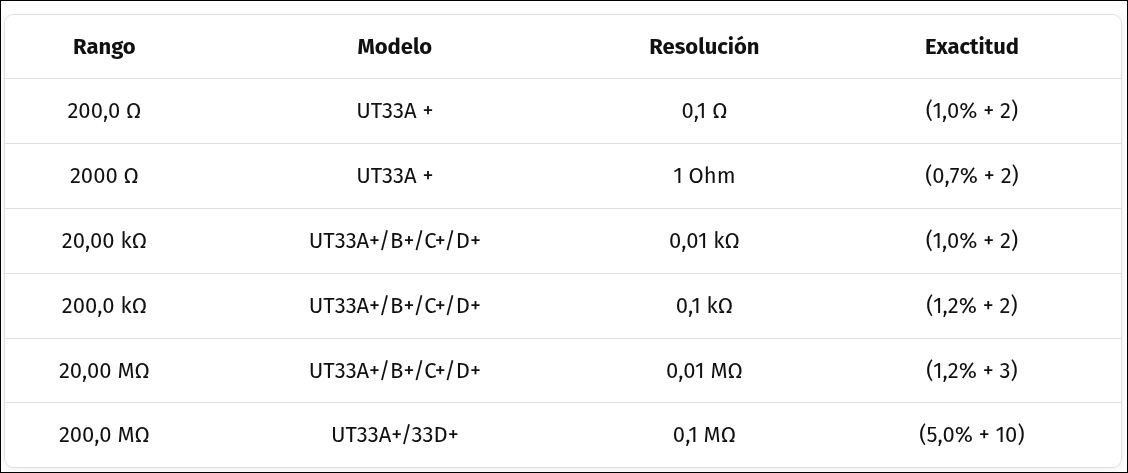
\includegraphics[width=0.8\textwidth]{images/tabla_presición_mult_unit.jpg}
    \caption{Especificaciones y precisión del multímetro UNI-T.}
    \label{fig:tabla_precision_mult_unit}
\end{figure}

